
\part[Exercícios extras]
{Exercícios extras}


\chapter[Exercícios extras]
{Exercícios extras}



\section*{Resumo}

Este capítulo reúne uma bateria de exercícios envolvendo todos os capítulos abordados durante o livro.

\section*{Problemas}
\begin{enumerate}
\item
  A partir de um ponto no mapa, simule um geiser inundando o terreno montanhoso com água. Considere que:
  \begin{itemize}
  	\item O terreno é construído randomicamente, onde sua altura varia entre 0 à 255.
  	\item Se valor da altura igual a 0, o terreno é verde puro. Se for maior que 0, ele varia sua coloração de vermelho de modo que, ao atingir valor de altura 255, sua cor seja amarelo puro.
  	\item A cada iteração, o valor de água sobe 10 unidades e espalha-se igualmente entre o terreno.
  \end{itemize}
  \label{ex:cap05_ex1}

  \begin{figure}[H]
    \centerline{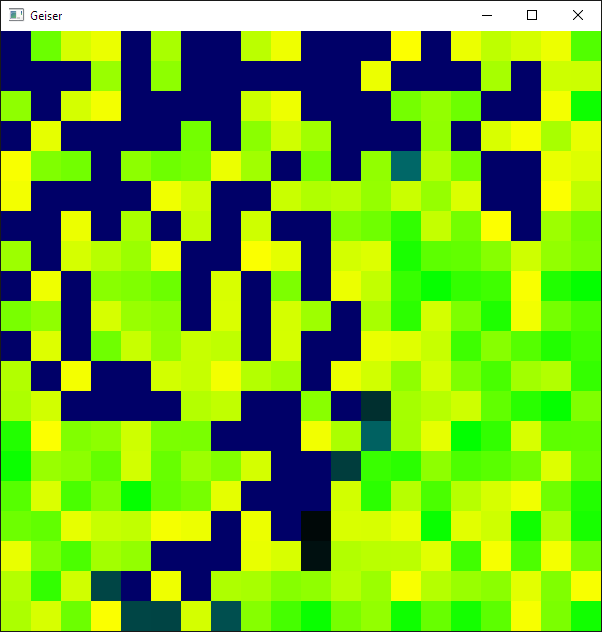
\includegraphics[width=.5\textwidth]{img/cap5_ex18.png}}
    \caption{Simulador de inundação}
    \label{fig:cap04_ex1}
  \end{figure}

\item
	Faça uma animação onde a lua está em órbita espiral em direção à terra. Ao atingir a terra, esta é jogada para fora da tela.
\label{ex:cap05_ex2}

  \begin{figure}[ht]
    \centerline{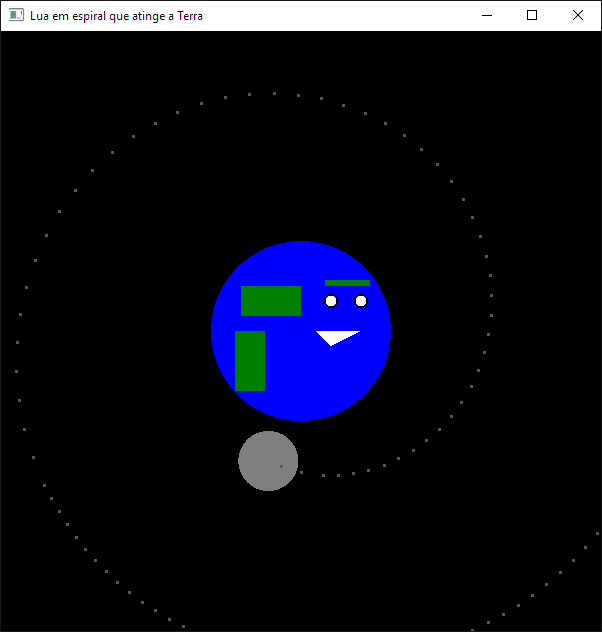
\includegraphics[width=.5\textwidth]{img/cap5_ex19.png}}
    \caption{Lua em órbita espiral}
    \label{fig:cap04_ex1}
  \end{figure}

\item
	Faça uma animação onde simule o funcionamento de um sonar, com os seguintes aspectos:
	\begin{itemize}
  	\item Há três seres na cena: um alienígena, um caça e um ruído.
  	\item O ruído realiza uma trajetória de um 8 deitado, $\infty$. Quando o ruído se aproxima do centro $(0,0)$ do sonar, ele desaparece, reaparecendo na tela depois de um certo tempo.
  	\item O caça realiza trajetória descrito pela Equação \ref{eq:cap05_ex3_1}.
  	\begin{equation}\label{eq:cap05_ex3_1}
  	\left\{\begin{matrix}
	 50 \cos(\alpha)\sqrt{2\cos(2\alpha)} & = x \\ 
	 50 \sin(\alpha)\sqrt{2\cos(2\alpha)} & = y
	\end{matrix}\right.
  	\end{equation}
  	Onde $\alpha$ é incrementado durante o loop.
  	\item O alienígena começa seu movimento, $dir$ indo da esquerda para direita. Enquanto $\alpha$ é incrementado a cada iteração do loop, há um $\theta$ que irá variar entre $0$ e $4\pi$. Toda vez que $\theta$ atingir $4\pi$, $\theta$ começa a variar de $0$ e $4\pi$ novamente, invertendo a direção $dir$ do alienígena.
  	Sendo assim, a trajetória do alienígena é descrita pela Equação \ref{eq:cap05_ex3_2}.
  	
  	\begin{equation}\label{eq:cap05_ex3_2}
  	\left\{\begin{matrix}
	 200 \cos(\theta \times dir)\div \theta\times dir & = x \\ 
	 200 \sin(\theta \times dir)\div \theta\times dir & = y \\ 
	\end{matrix}\right.
  	\end{equation}

  \end{itemize}
\label{ex:cap05_ex3}

  \begin{figure}[ht]
    \centerline{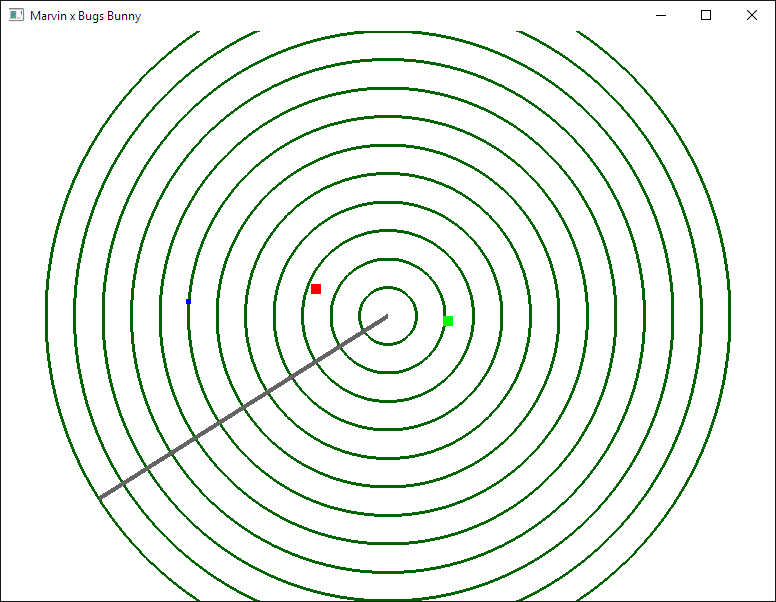
\includegraphics[width=.5\textwidth]{img/cap5_ex20.png}}
    \caption{Sonar}
    \label{fig:cap04_ex1}
  \end{figure}
\end{enumerate}

\section*{Soluções}

\subsection*{Exercício \ref{ex:cap05_ex1} }

\lstinputlisting[caption=Simulador de inundação, style=customc, label=lst:cap5_ex1]{src/ex18_geiser.cpp}

\subsection*{Exercício \ref{ex:cap05_ex2} }

\lstinputlisting[caption=Lua em órbita espiral, style=customc, label=lst:cap5_ex2]{src/ex19_luaespiral.cpp}

\subsection*{Exercício \ref{ex:cap05_ex3} }

\lstinputlisting[caption=Sonar, style=customc, label=lst:cap5_ex2]{src/ex20_sonar.cpp}